\documentclass{standalone}
\usepackage{tikz}
\usetikzlibrary[arrows,positioning,matrix]

\begin{document}
\begin{tikzpicture}
  \node[draw=none] (randomspeedprofile) {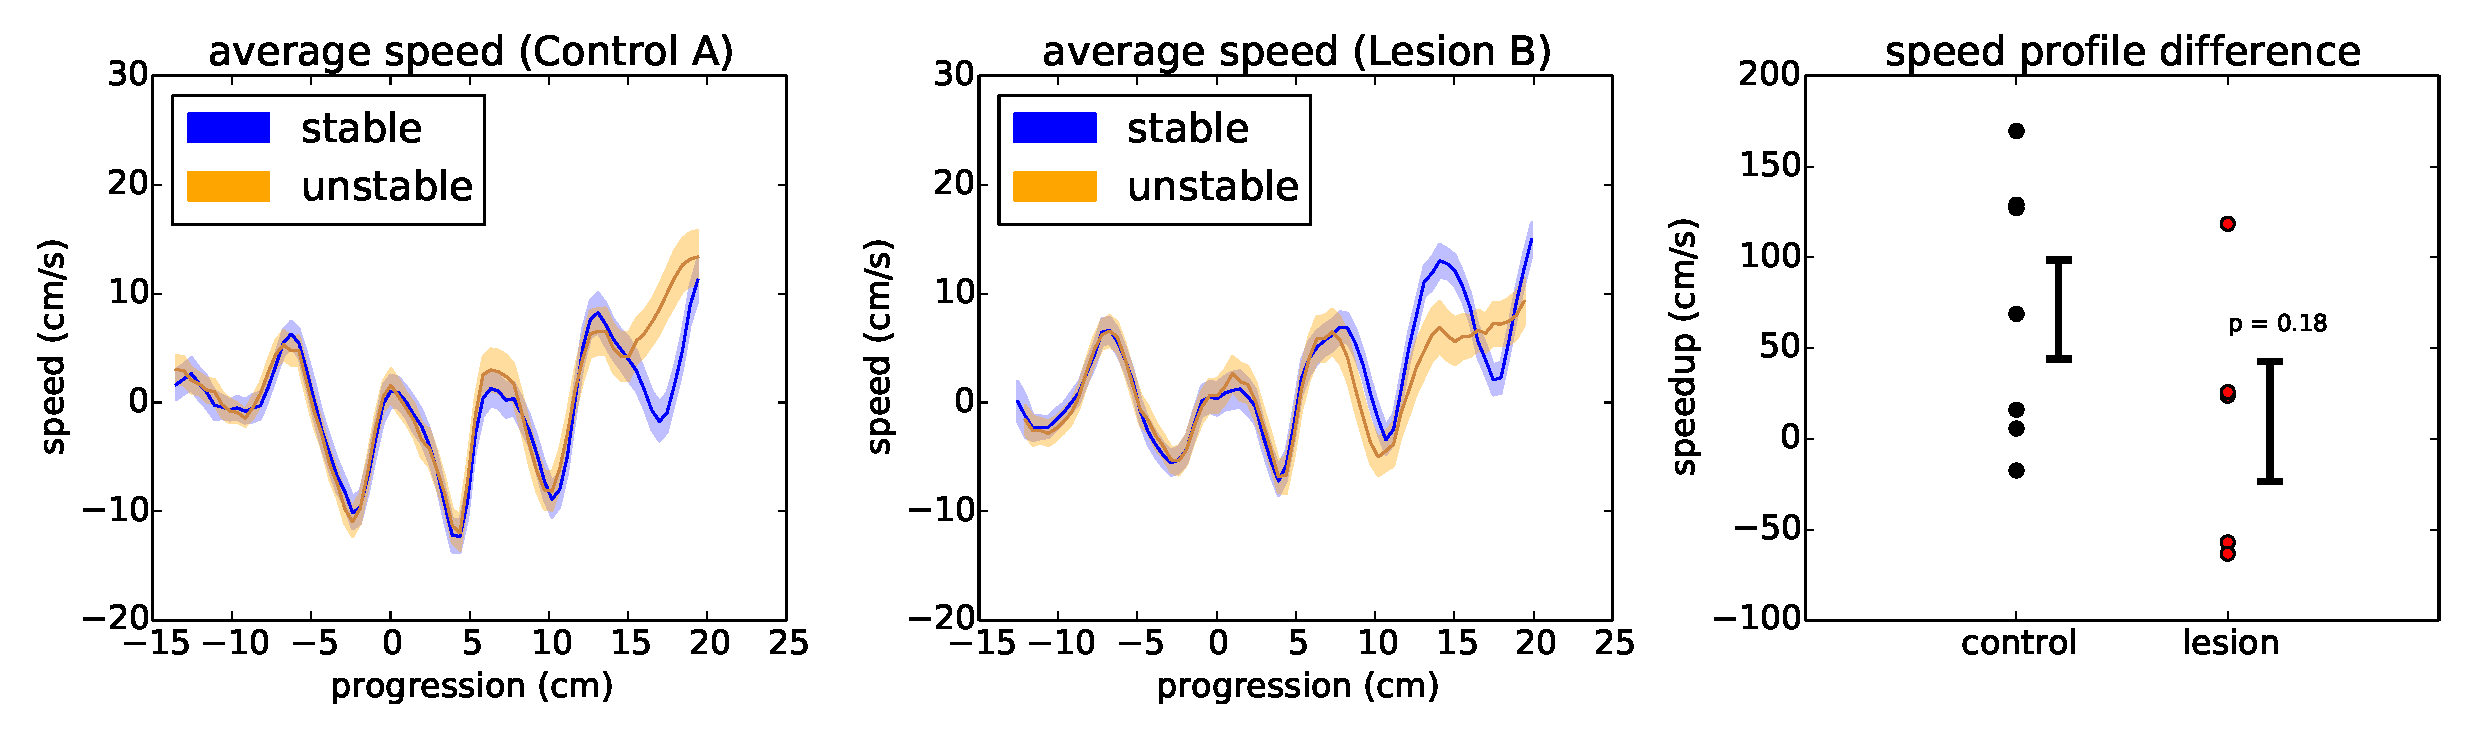
\includegraphics[width=1.1\textwidth]{elements/randomspeedprofile}};
  \node[draw=none,above left=-3mm and -7mm of randomspeedprofile] (A) {A};
  \node[draw=none,above left=-3mm and -51mm of randomspeedprofile] (B) {B};
  \node[draw=none,above left=-3mm and -94.5mm of randomspeedprofile] (C) {C};
\end{tikzpicture}
\end{document}